
%---------------------------------
\subsubsection{What is the geoid?}



The geoid is usually defined in two ways:
\begin{itemize}
\item Mean sea level (easy to define in the oceans, but harder on land)
\item A gravitational equipotential surface. This means that everywhere at sea level experiences the same value of gravity potential, so there is no tendency for water to flow downhill since all points in the vicinity have the same value of gravity potential, pointed toward the center of the earth.
\end{itemize}

\begin{center}
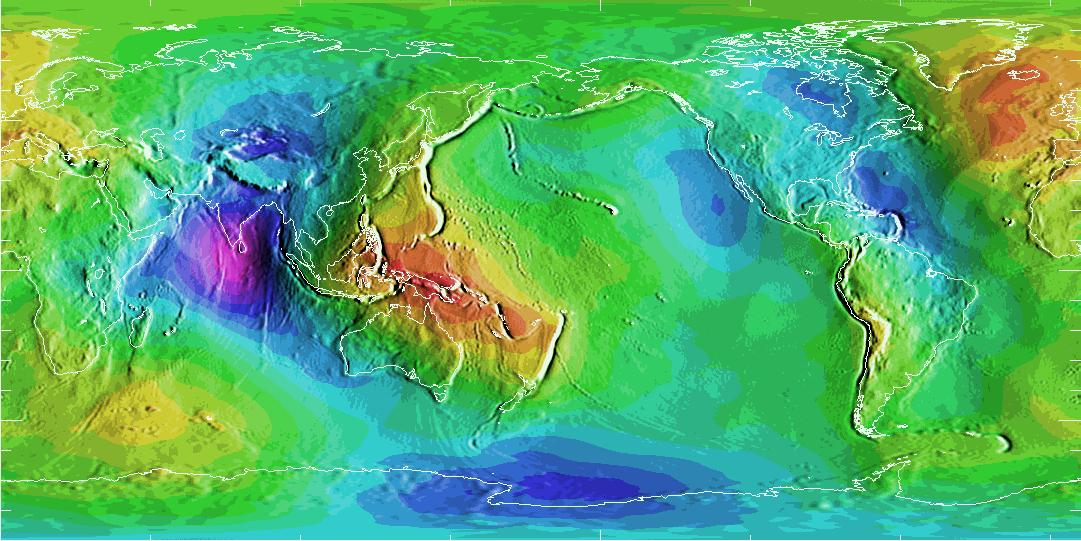
\includegraphics[width=10cm]{images/geoid/ww15mgh}\\
{\captionfont Data Max value: 85.4 meters, east of New Guinea. Data Min value:-107.0 meters, south of India. 
This image shows 15'x15' geoid undulations covering the planet Earth from the NIMA/GSFC WGS-84 EGM96 15' Geoid Height File. The undulations refer to the differences from the WGS-84(G873) reference ellipsoid. Map and description from National Geodetic Survey.}
\end{center}
%https://www.usna.edu/Users/oceano/pguth/md_help/geology_course/geoid.htm


%---------------------------------
\subsubsection{How to compute it?}

%---------------------------------
\subsubsection{Interesting modelling}

\begin{center}
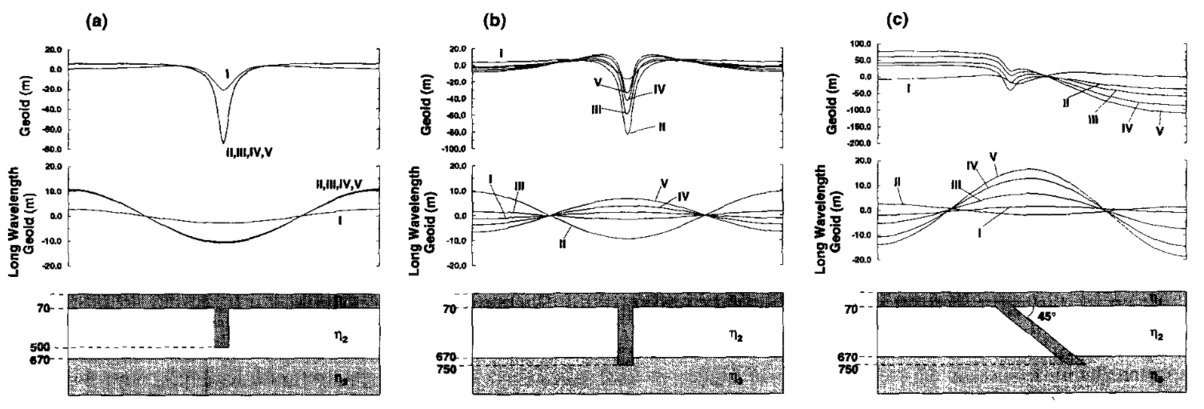
\includegraphics[width=15cm]{images/geoid/mogu96}
{\scriptsize Idealized 2D slab calculations for each viscosity model: geoid and geoid filtered 
to pass only the longest wavelengths ($\sim$ 4000 km).
(a) Cold slab extends to 500 km depth in the upper mantle, 
(b) Slab extends to 750 km so that it is partly supported by the high viscosity lower mantle at 670 km. 
(c) Slab tilted at 45\degree to the vertical extending to the top of the lower mantle. 
Taken from \cite{mogu96}}
\end{center}
